\section{Integration at the transfer level}

\subsection{Integrating FDT into PhEDEx}
The FDT\footnote{Fast Data Transfer (fdt.cern.ch)} tool integrates IDCP
\footnote{InterDomain Controller Protocol} (OSCARS)
\footnote{On-Demand Secure Circuits and Advance Reservation System} calls so
integrating it in PhEDEx naturally gives us BoD\footnote{Bandwidth on Demand}
capabilities. In addition to this, we discovered that FDT performs extremely well
as a transfer tool in itself, as we will show in this paper.

As shown in Figure \ref{fig:PhEDEx-FDT-arch}, the current architecture consists
of four main components:
\begin{description}
	\item[FDT tool] - written in Java it's based on an asynchronous, flexible 
multithreaded system, using the capabilities of the Java NIO\footnote{New I/O} 
libraries. It's capable of reading and writing at disk speed over wide area 
networks and runs on all major platforms. 
	\item[PhEDEx backend*] - written in Perl, this backend
receives transfer jobs from the FileDownload site agent which will in turn 
invoke the fdtcp wrapper. 
	\item[Fdtcp wrapper*] - written in Python this is the 
interface between PhEDEx and FDT. It prepares the file list as required by FDT, 
invokes the fdtd service and harvests reports to be propagated back to PhEDEx.
	\item[Fdtcp daemon*] - written in Python as well, it's 
a permanently running daemon, in charge with authentication and completion of requests 
from fdtcp. These requests are transmitted via PYRO\footnote{PYthon Remote Objects} 
calls and will either launch the FDT in client mode on source sites or FDT in server 
mode on destination sites.
\end{description}

The components marked with * were not developed by the same team as the one responsible 
for FDT.

\begin{figure}[h]
  \centering
  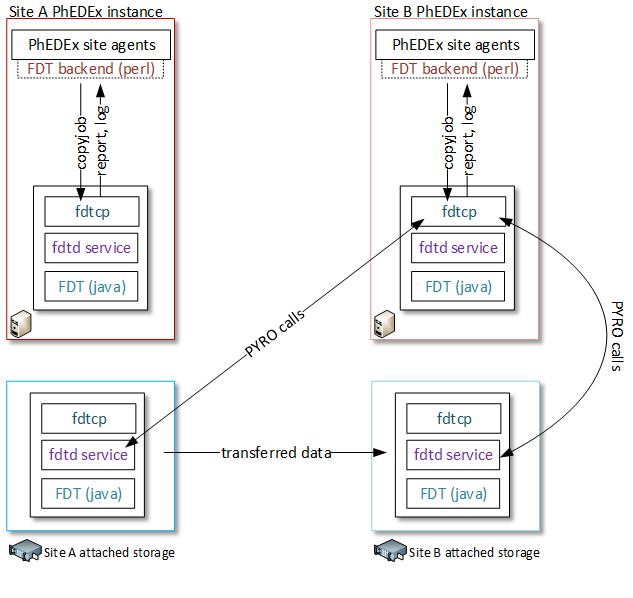
\includegraphics[width=0.95\textwidth]{Figures/PhEDEx-and-FDT-diagram.png}
  \caption{Diagram of various components needed to integrate FDT into PhEDEx}
  \label{fig:PhEDEx-FDT-arch}
\end{figure} 

Figure \ref{fig:PhEDEx-FDT-arch} also describes a normal scenario in which Site B
needs to transfer data from Site A. In this example, the PhEDEx instance and the
storage node are separate physical servers. 

Once the FileDownload agent on the PhEDEx server on Site A, marks all the files as
ready for transfer, the FDT backend on that machine will then issue an fdtcp 
command with the list of files that needs to be copied from the storage node of
Site A to the storage node of Site B.

Fdtcp will in turn, invoke the fdtd daemons on the two storage nodes. Each fdtd
daemon will first verify that the command comes from an approved server, after
which it will then launch the appropriate FDT tool. The fdtd daemon on Site B 
will start the FDT tool in server mode and the daemon on site B starts FDT in 
client mode.

Once this is done, the transfers are handled by FDT. After the transfer finishes
the reports are then propagated up the chain, eventually reaching PhEDEx.

\subsection{Setup and transfer results with FDT}

\subsubsection{Setup}

The tests were run on our setup (Figure \ref{fig:ANSE-setup}), using the Geneva
(T2\_ANSE\_Geneva) and Amsterdam (T2\_ANSE\_Amsterdam) sites. All LSI controllers
were used.

Each transfer job was 2.25TB (150x15TB files).

\subsubsection{Transfer results with FDT}

As seen in Figure \ref{fig:FDT-Transfers} and Figure \ref{fig:FDT-Transfers-PhEDEx}
FDT is able to achieve sustained rates of over 1500MB/sec. As PhEDEx shows,
the average sits at a marginally slower 1360MB/sec. As visible in 
Figure \ref{fig:FDT-Transfers}, the plot has periodical drops in transfer rates.
This is due to the fact that between each transfer job (which is composed of a limited
number of files) there is a delay between the ending of one job and the launch of
a new one. This is what accounts for the difference in average reported rates by PhEDEx
and the average rate for each transfer job.

These high transfer rates are not only due to the storage system alone... FDT 
automatically starts the correct number of readers and writers if the files at 
the source and destinations sites are spread on different physical disks/controllers.

\begin{figure}[h]
  \centering
  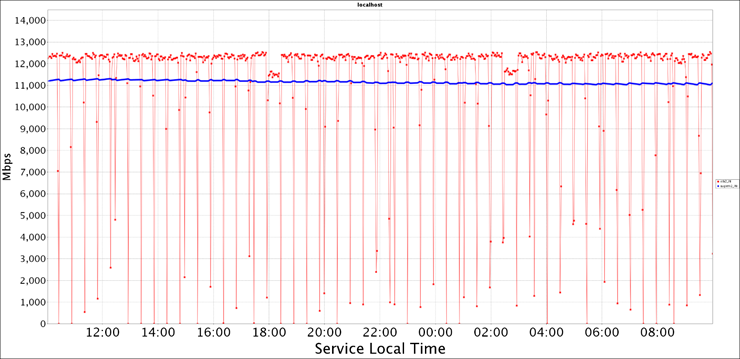
\includegraphics[width=0.95\textwidth]{Figures/FDT-transfers.png}
  \caption{PhEDEx transfers over 24hrs using FDT - MonALISA plot}
  \label{fig:FDT-Transfers}
\end{figure} 

\begin{figure}[h]
  \centering
  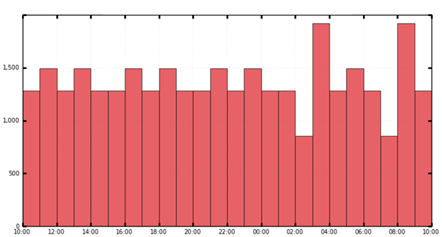
\includegraphics[width=0.95\textwidth]{Figures/FDT-transfers-PhEDEx.png}
  \caption{PhEDEx transfers over 24hrs using FDT - PhEDEx plot (in MB/sec)}
  \label{fig:FDT-Transfers-PhEDEx}
\end{figure} 


\subsubsection{Caveats}

At the moment this system does have some drawbacks:

\begin{itemize}
	\item This setup is not used by anyone in production at the moment
	\item FDT requires a POSIX compatible interface to function. At the moment
not all PhEDEx sites are capable of exposing that.
	\item In order to get the best performance out of the systems, files that
are to be transfered need to be spread among different disks on both source
and destination storage servers. This puts an additional configuration effort
on the sites and adds more complexity in the TFCs\footnote{Transfer File
Catalogs}
\end{itemize}